\documentclass[conference]{IEEEtran}
\usepackage{amssymb,amsmath,amsthm}
\usepackage{algorithm}
\usepackage{algpseudocode}
\usepackage{graphicx}
\usepackage{caption}
\usepackage{cite}
\usepackage{sidecap}
\usepackage{lipsum}

\usepackage[dvipsnames]{xcolor}
\colorlet{lhue}{SpringGreen}
\colorlet{mhue}{WildStrawberry}
\colorlet{ghue}{CornflowerBlue}
\colorlet{vhue}{Goldenrod}
\usepackage[textsize=small,textwidth=15mm]{todonotes}
\setlength{\marginparwidth}{15mm}
\newcommand{\NDT}[1]{\todo[bordercolor=ghue,linecolor=ghue,color=ghue!40]{Tias: #1}}
\newcommand{\NDTi}[1]{\todo[inline,bordercolor=ghue,color=ghue!40]{Tias: #1}}
\newcommand{\NDB}[1]{\todo[bordercolor=mhue,linecolor=mhue,color=mhue!40]{Behrouz: #1}}
\newcommand{\NDBi}[1]{\todo[inline,bordercolor=mhue,color=mhue!40]{Behrouz: #1}}

\newtheorem{theorem}{Theorem}
\newtheorem{definition}{Definition}

\begin{document}

\title{A Branch-and-Cut Algorithm for Constrained Graph Clustering}

\author{\IEEEauthorblockN{Behrouz Babaki}
\IEEEauthorblockA{Dept. Computer Science\\
KU Leuven, Belgium}
\and
\IEEEauthorblockN{Dries Van Daele}
\IEEEauthorblockA{Dept. Computer Science\\
KU Leuven, Belgium}
\and
\IEEEauthorblockN{Tias Guns}
\IEEEauthorblockA{Dept. Computer Science, KU Leuven, Belgium \\ \&
Dept. Business technology and Operations, \\VUB, Belgium}}

\maketitle

\begin{abstract}
Clustering is a well-defined problem class in data mining, and many variations of it exists. However, practitioners often have additional constraints or quality scores that are not supported by standard algorithms. This has lead to the study of constrained clustering, which investigates generic methods to handle a variety of constraints and objectives. In our bioinformatics work, we were faced with exactly such a problem: a graph clustering problem with strict connectivity requirements and an objective function based on penalties rather than density of the clustering. In this paper, we explain the problem including the constraints and quality measures, and propose to use generic Mixed Integer Programming to solve it. We propose two approaches to handle the connectivity requirement in particular: one defined over all simple paths in the graph explicitly, and one based on cutting planes that enforce connectivity only if needed. Our experiments show that these approaches are able to solve the problem well. We hence demonstrate the applicability of generic OR methods on this application-driven data mining problem.
\end{abstract}

\section{Introduction}
\label{introduction}

% graph clustering (and partitioning)
Clustering is the task of partitioning a set of instances into
homogeneous subsets. The quality of the clustering is typically determined by the \textit{distance} between the instances. In graph clustering~\cite{schaeffer2007graph}, each instance is assumed to a node in a graph; this graph is typically not fully connected. The quality is then determined by the \textit{density} of the instances within a cluster or by the \textit{cut size} between the clusters, that is the number of edges shared between different clusters. The latter is for example frequently studied in the field of graph partitioning~\cite{BulucMSS016}. Graph clustering has applications in many domains including social network analysis and community detection, information networks, transportation and logistics, and bioinformatics~\cite{schaeffer2007graph}.

% constrained clustering
As data mining is increasingly applied on more and more problems in different domains, it increasingly happens that existing clustering methods are not suited for the problem at hand. This is either because the problem domain imposes additional constraints that can not be expressed in these methods, or because the objective function has a non-standard form. This has lead to the field of \textit{constrained clustering}, which studies clustering problems involving different constraints and objectives~\cite{basu2008constrained}. An increasingly popular way to handle a broad range of constraints and objectives is to use generic optimisation tools. In other words, to cast the problem as an optimisation problem and to use generic (discrete) optimisation solvers such as constraint programming~\cite{DaoDV13}, mixed integer programming~\cite{DBLP:conf/aaai/GilpinND13,DBLP:conf/cpaior/BabakiGN14} or maximum satisfiability solvers~\cite{DBLP:journals/ai/BergJ17}. Though scalability can be an issue, these solvers can intrinsically handle different objectives and constraints.

% bio problem (interaction & co-occurence + size)
The problem we study in this paper is such a graph clustering problem that does not fit existing approaches. It is part of a bigger pipeline in computational cancer research, where the goal is to find \textit{pathways} in gene interaction networks. There is hence an \textit{interaction network} and it is a hard constraint that all nodes belonging to a cluster must be connected in this interaction network. To evaluate the quality there is a separate weighted \textit{co-occurence} network and the nodes belonging to a cluster should have a low co-occurence penalty. Furthermore, small pathways are biologically less meaningful and hence the size of the clusters should also be maximized. The problem is hence a bi-objective graph clustering problem with hard connectivity constraints on a separate network. Existing methods are not able to handle such a complex setting, hence we study a mixed integer programming approach.
%This perspective encourages formulating
%data mining problems as models in constraint satisfaction/optimization
%frameworks (e.g. constraint programming and integer programming). One
%of the motivations for doing so is that existing algorithms can be
%extended to new problems by modification of addition of constraints.

% contributions
More specifically, are contributions are as follows: 1) we identify a new bi-objective constrained graph clustering with applications in bio-informatics and present a MIP formulation of the problem; 2) to better handle the large number of connectivity constraints, we propose a branch-and-cut approach that adds connectivity constraints as needed using the principle of node-cut sets. Our experiments demonstrate the effectiveness of the approach.

The rest of this paper is structured as follows:  In
section~\ref{sec:motivation} we present the application that motivates
this problem.  Section~\ref{sec:definition} introduces the formal
problem definition and a MIP formulation with the connectivity requirement.
In section~\ref{sec:connectivity} we introduce two methods for handling the connectivity requirement, including a cutting plane approach. Section~\ref{sec:experiments} contains the experiments, followed by related work in section~\ref{sec:related} after which we conclude.


\section{Motivating application}
\label{sec:motivation}
In cancer research, tumor tissue is collected from patients for further study. Such a tumor is basically a cell in which one or more genes have mutated. Normally that cell would be destroyed by the immune system, but in case of a tumor that cell has managed to survive and may even be growing (out of control).
Genes and mutated genes can be identified in a tumor by sequencing the DNA of the tissue. Nowadays, this sequencing has become fairly commonplace, enabling the genome-wide measurement of mutated genes across large groups of cancer patients.

The key challenges when interpreting these data are to detect the (mutated) genes that affect the creation and development of cancer and to gain an understanding of their interaction. Initially, the main focus by the community was solely on the detection of key driver genes. However, there are typically many mutated genes making it challenging to detect rare ones with high statistical significance. For this reason, there is recently a rise in methods aiming to exploit the information contained in the human interaction network \cite{some_methods}. This network expresses which genes interact with each other. This can be used to verify that a set of genes interact with each other.

In our setting we start by considering a subgraph of the human interaction network containing only those genes and interactions that were identified as being highly relevant to a particular cancer. Each node represents a gene or gene product, and each edge represent an interaction between a pair of nodes. The graph may consist of multiple connected components. It is our goal to separate distinct \textit{pathways} from each of these components, where a pathway is a set of genes that interact with each other.

By incorporating such biological pathway information, a superior selection and understanding of genes and their interactions is possible. %These new methods do introduce novel challenges. We notice that the underlying mechanisms that affect individual patients are not always easily distinguishable from the extracted subgraphs. More specifically, it is the case that the pathways contained in these subgraphs may be connected to one another or even overlap.
%
A difficult challenge however is how to determine that two genes are more likely to belong to the same or to a different pathway. Fortunately, it is known that the creation and growth of tumors follows a clonal \textit{evolutionary} model. Following this model, it is unlikely that within a single pathway a tumor would disrupt and mutate different genes. Indeed, it is sufficient to disrupt one gene to disrupt the pathway, and hence evolutionarily there is little intensive to disrupt others as well. As a consequence, it is less common that multiple mutated genes of a single pathway are observed within the same patient. We can hence compute a co-occurrence penalty score for each pair of genes, based on the harm associated with the mutations and the number of patients in which that pair was observed.

While obtaining pathways with a low penalty is important, one should not go as far as dividing each gene into small clusters. For this reason, we will aim to balance the size of the (smallest) pathway with the amount of penalty the pathways incur.



\begin{figure}
\centering
\begin{minipage}{.3\linewidth}
\centering
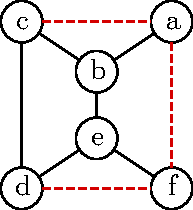
\includegraphics[scale=0.6]{images/interaction}
\end{minipage}%
\begin{minipage}{.3\linewidth}
\centering
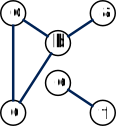
\includegraphics[scale=0.6]{images/interaction_no_overlap}
\end{minipage}%
\begin{minipage}{.4\linewidth}
\centering
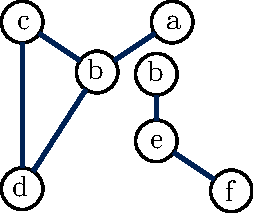
\includegraphics[scale=0.6]{images/interaction_overlap}
\end{minipage}
\captionsetup{font=small,margin=10pt}
\captionof{figure}{(left) A small subgraph extracted from the interaction network. Dashed lines represent the can-not-link constraints. (middle) the pathways obtained from non-overlapping clusters (right) the pathways obtained from overlapping clusters.}
\label{fig:minimal}
\end{figure}


\section{Problem definition}
\label{sec:definition}

We assume that the reader is familiar with basic graph theory. Here we quickly review some important basic notions: A graph $G=(V, E)$ consists of a set of nodes $G$ and a set of edges $E$. A graph is \emph{simple} if it does not have any loops or double edges. A graph is \emph{connected} if there is a path between each pair of its nodes. The nodes on a path except the first and last ones are called the \emph{intermediate nodes}. A \emph{simple path} is a path with no cycles. The induced subgraph of $G$ on a set of nodes $W$ has $W$ as its node-set and contains those edges in $G$ which have both endpoints in $W$. 


%containing only those genes and interactions that were identified as being highly relevant to a particular cancer. 
% Each pathway is connected, thus motivating the usage of connectivity constraints. The rule that pairs of mutated genes within individual patients should not be assigned to the same pathway can be imposed using can-not-link constraints. Since there are several known exceptions to this rule, we require the usage of soft constraints. The penalty associated with violating such a constraint is a function of the harm associated with the mutations and the number of patients in which that pair was observed.


Consider a simple undirected graph $G=(V, E)$ where nodes represent genes, and edges represent interactions between those genes. Our goal is to partition $V$
into $k$ subsets (called \emph{clusters} from now on), such that the
subgraph induced by each subset is connected. These represent the pathways we seek to identify. Our preference is to avoid
having clusters that contain only a small number of nodes. To enforce
this preference, we define one of our goals as maximizing the size of
the smallest cluster. Moreover, there exists a set of tuples
$C = \{(u, v, w): u, v \in V, w \in \mathbb{R}^+\}$ which indicates that
including $u$ and $v$ in the same cluster will induce a penalty of $w$. We denote all edges $(u, v)$ such that $(u, v, w) \in C$ by $E_C$. Our second goal is to minimize the sum of such penalties.


To include both goals in the objective function, assume that $S$ is the
size of the smallest cluster and $W$ is the total penalty. We define the
objective function as maximizing $S - \gamma W$ where $\gamma$ is a
positive parameter specified by user which determines the relative importance of each of the two goals.
\NDB{Mention normalization}

We can formulate this problem as an integer linear program. The main
decision variables in this formulation are those that determine the
assignment of nodes to the clusters. In our formulation, the binary
variable $x_{ij}$ indicates whether or not node $i$ is included in
cluster $j$. We know that each node is assigned to exactly one
cluster. This can be enforced by the following set of constraints:

\begin{equation}
\sum_{j=1}^k x_{ij} = 1 \quad \forall i \in \{1, \ldots, |V|\} \label{cons:assign}\\
\end{equation}

To include the penalties in the model, we introduce additional
variables. The binary variable $y_{uvj}$ is equal to one if and only if
nodes $u$ and $v$ are both included in the $j$th cluster. To enforce
this property, we add the following constraints to the model:

\begin{equation}
y_{uvj} \geq x_{uj} + x_{vj} -1 \quad \forall j \in \{1, \ldots, k\}, \forall (u, v) \in E_{C}
\end{equation}

If both $x_{uj}$ and $x_{vj}$ are equal to one, this constraint forces
$y_{uvj}$ to be equal to one. Otherwise, $y_{uvj}$ can be either zero or
one. However, as we will see, $y_{uvj}$ is included in the objective
function with a negative coefficient. Hence the optimization procedure
will automatically fix $y_{uvj}$ to zero in such cases.

Finally, we introduce an integer variable $s$ which represents the size
of the smallest cluster. The domain of $s$ is
$\{0, \ldots, \lfloor \frac{|V|}{k} \rfloor \}$. The following constraints
ensure that $s$ represents the size of the smallest cluster:

\begin{align}
s \leq \sum_{i=1}^{|V|} x_{ij} \quad \forall j \in \{1, \ldots, k\}
\end{align}

Our formulation so far does not ensure that the nodes in each cluster
are connected. For now assume that constraint
$\mathsf{connected}(x_{1j}, \ldots, x_{|V|j})$ enforces the connectivity of
cluster $j$. We will discuss the exact formulation of this constraint in
the next section. 

The model that we defined in this section is presented
below:

\begin{align}
& \text{maximize} \quad s - \gamma \sum_{j=1}^{k} \sum_{(w, u, v) \in C} w  y_{uvj}  \\
&\textit{s.t.}                                                                       \nonumber \\
&\sum_{j=1}^k x_{ij} = 1                                                             \forall i \in \{1, \ldots, |V|\} \\
& y_{uvj} \geq x_{uj} + x_{vj} -1                                                    \forall j \in \{1, \ldots, k\}, \forall (u, v) \in E_{C} \\
& s \leq \sum_{i=1}^{|V|} x_{ij}                                                     \forall j \in \{1, \ldots, k\} \\
& \mathsf{connected}(x_{1j}, \ldots, x_{|V|j})                                       \forall j \in \{1, \ldots, k\} \\
& x_{ij} \in \{0, 1\}                                                                \forall j \in \{1, \ldots, k\}, \forall i \in \{1, \ldots, |V|\} \\
& y_{uvj} \in \{0, 1\}                                                               \forall j \in \{1, \ldots, k\}, \forall (u, v) \in E_{C} \\
& s \in \{0, \ldots, \lfloor \frac{|V|}{k} \rfloor \}                                  
\end{align}

\section{Extensions and improvements}
\NDBi{We can collect the following into a new section}

\subsection{Overlapping clusters}
Sometimes we can allow a node to be included in more than one cluster. For example, in our motivating application it is the case that a gene can serve as an essential part of different pathways. 

To modify our formulation to allow for overlapping clusters we need to ensure that each node is included in \emph{at least} one cluster. To apply this modification to our formulation, we only need to replace constraints~\ref{cons:assign} with the following inequalities:

\begin{equation}
\sum_{j=1}^{k} x_{ij} \geq 1 \qquad i \in \{1, \ldots, |V| \}
\end{equation}

\subsection{Breaking the symmetries}
Clustering problems often have an inherent symmetry which is due to the fact that the labels of clusters are arbitrary. This means that for each solution, there are $k!$ equivalent solutions that only differ by the cluster labels. We can strengthen our formulation by breaking these symmetries. \cite{SheraliD05a} suggests two options to reduce these symmetries: 1) Assign label one to the cluster that contains node one. 2) Assign labels to other clusters in the increasing order of their sizes. This translates to the following constraints:

\begin{align}
&x_{11} = 1 \\
&\sum_{i=1}^{|V|} x_{ij} \leq \sum_{i=1}^{|V|} x_{i,j+1} \qquad j \in \{2, \ldots, k\}
\end{align}

These constraints do not eliminate all symmetries (especially in the case of overlapping clusters) but still lead to improvements in performance in practice. 

\subsection{Obtaining the set of Pareto optimal solutions}
An alternative to setting a trade-off between the two conflicting objectives is to compute the set of \emph{Pareto optimal} solutions. A solution of a bi-objective optimization problem is Pareto optimal if there is no other solution with a better quality with respect to both objectives. Obtaining the set of Pareto optimal solutions for other types of bi-objective constrained clustering has been studied before~\cite{GunsDVD16}. To obtain the Pareto optimal solutions, we use a method based on the $\epsilon$-constraint algorithm~\cite{DBLP0015143}. We remove the size of the smallest cluster from the objective and bound it by a hard constraint. Then we iteratively solve this modified problem, each time using a bound that is one higher than the size of the smallest cluster in the previous solution (algorithm~\ref{alg:pareto}).

\begin{algorithm}
\centering
\caption{Computing the set of Pareto optimal solutions}
\label{alg:pareto}
\begin{algorithmic}[1]
\State $\mathcal{P} \gets \emptyset$ \Comment{the set of Pareto optimal solutions}
\State $min\_size \gets 0$
\Repeat
	\State $solution \gets \textsc{MinimizePenalties}(G, W, min\_size)$
	\State $\mathcal{P} \gets \mathcal{P} \cup solution$
	\State $s \gets$ size of the smallest cluster in $solution$
	\State $min\_size \gets s+1$
\Until{no $solution$ was found}
\end{algorithmic}
\end{algorithm}

\NDTi{possible story: 1) ensure connectedness: must be a path between two coclustered poins; 2) cutting plane is generate when violated. Generating 17 requires adding 16's too. Instead, can use relation between connectedness and node-cuts. Using node-cuts in constraints is over variables directly. Number of node-cuts is worst-case exponential, but one violated one is sufficient to invalidate a solution so can generate one as cutting plane. Which one? For integer values does not matter: any violated one. Common approach to finding node-cuts is using a flow problem. Can use this here as follows... Advantage of solving flow problem is that also applicable to real-valued xs. Hence algorithm is...}
\section{Enforcing connectivity}
\label{sec:connectivity}

In this section we give a concrete definition of the constraint $\mathsf{connected}(x_{1j}, \ldots, x_{|V|j})$. For a cluster to be connected, for each pair of points belonging to the cluster there should exist at least one path between these two nodes such that all nodes on this path also belong to this cluster. In section~\ref{sec:enumerate} we enforce this condition by explicitly enumerating all simple paths between each pair of non-adjacent nodes in the graph and adding variables and constraints for these paths. However, the exponential number of added constraints and variables limits the scalability of this method.

Despite the exponential number of constraints, given an objective function it is likely that only a manageable subset of these constraints are active at the optimal solution. The \emph{cutting plane} algorithm is a method that tries to approximate this subset incrementally. In section~\ref{sec:bnc} we introduce another formulation for the connectivity constraint which again amounts to an exponential number of linear constraints, but lends itself better to the requirements of the cutting plane method.

\subsection{Enumerating all simple paths}
\label{sec:enumerate}

Consider a simple path between the nodes $u$ and $v$. Let $I$ denote the set of indices of the intermediate nodes on this path. Assume that binary variable $y$ indicates that all these nodes belong to cluster $j$. A standard translation of the relation $(y=1) \Leftrightarrow \land_{i \in I} (x_{ij}=1)$ to linear constraints gives the following inequality:

\begin{equation*}
0 \leq \sum_{i \in I} x_{ij} - |I|y \leq |I|-1
\end{equation*}

More formally, let $P_{uv}$ denote the set of all simple paths between nodes $u$ and $v$. For a path $P_r \in P_{uv}$, let $I_r$ denote the set of indices of intermediate nodes of $P_r$. We introduce binary variable $y_{rj}$ to indicate that all these nodes are assigned to cluster $j$. This relationship is enforced by the following constraints:
\begin{multline}
0 \leq \sum_{i\in I_r} x_{ij} - |I_r| y_{rj} \leq |I_r| - 1 \\
\forall j \in \{1, \ldots, k\}, \forall u, v \in V, (u, v) \notin E, \\ \forall r \in \{1, \ldots, |P_{uv}|\}
\label{cons:path}
\end{multline}

Finally, to enforce the condition $(x_{uj}=1 \land x_{vj}=1) \Rightarrow \lor_{r} (y_{rj}=1)$, we add the following constraints to the model:

\begin{multline}
x_{uj} + x_{vj} -1 \leq \sum_{r=1}^{|P_{uv}|} y_{rj} \\
\forall u, v \in V, (u, v) \notin E, \forall j \in \{1, \ldots, k\}
\label{cons:pconnect}
\end{multline}

\subsection{A cutting plane approach}
\label{sec:bnc}

 In the cutting plane method two steps are iteratively repeated: 1) A model that includes only a subset of the constraints is solved. 2) A constraint that is violated by the current solution is added to the model. These steps are repeated until no constraint is violated. To use the cutting plane algorithm, we need an oracle that given a vector $\mathbf{x}$ can check if $\mathbf{x}$ satisfies all constraints and if not, finds a constraint that is violated by $\mathbf{x}$. Since in the latter case the added constraint separates $\mathbf{x}$ from the feasible region, the problem solved by the oracle is called the \emph{separation} problem. In a ~\emph{branch and cut} algorithm, cutting planes are added throughout the branch and bound tree. Note that even if we add some or none of the cuts to the linear programming (LP) relaxation, it will still provide a valid bound. Hence it is possible to add the cuts only when an integer solution is obtained.

 
 Applying the cutting plane method to the formulation of section~\ref{sec:bnc} is not easy, since the $y$ variables in a constraint from the constraint set~\ref{cons:pconnect} couple it with an exponential number of constraints from the constraint set~\ref{cons:path}. Therefore we adopt the approach of ~\cite{CarvajalCGVW13} which defines the connectivity constraints in terms of \emph{node-cut sets}. The following definition and theorem are taken from~\cite{CarvajalCGVW13}.

\begin{definition}[Node-cut set]
Given nodes $u, v \in V$ that are not adjacent ($(u, v) \notin E$), a set of nodes $S \subseteq V \setminus \{u, v\}$ is a \emph{node-cut set} separating $u$ and $v$ (or simply a \emph{$uv$-node cut}) if all paths between $u$ and $v$ intersect $S$.
\end{definition}

A $uv$-node cut is \emph{minimal} if it is not a $uv$-node cut after removing any of its nodes. For a pair of non-adjacent nodes $u$ and $v$, we denote by $\Gamma(u, v)$ the set of all minimal $uv$-node cut sets. Figure~\ref{fig:cutset} shows examples of minimal node-cut sets. The following theorem relates the connectivity of a graph to its minimal node-cut sets. 

\begin{SCfigure}[1.2]
\centering
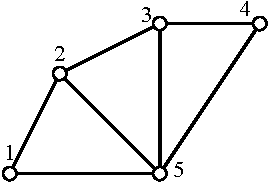
\includegraphics[scale=0.7]{images/cutset}
\captionsetup{font=small}
\captionof{figure}{The sets \{2, 5\} and \{3, 5\} belong to $\Gamma(1, 4)$, but the set \{2, 3, 5\} does not.}
\label{fig:cutset}
\end{SCfigure}

\begin{theorem}
Given $U \subseteq V$ and a pair of non-adjacent nodes $u, v \in U$, there exists a path between $u$ and $v$ in the subgraph induced by $U$ if and only if all $uv$-node cuts $S$ are such that $S \cap U \neq \emptyset$.
\label{theorem:cutset}
\end{theorem}

According to theorem~\ref{theorem:cutset} to ensure that cluster $j$ is connected, the following condition should hold for each $uv$-node cut $S$:

\begin{equation*}
(x_{uj}=1 \land x_{vj}=1) \Rightarrow \lor_{w \in S} (x_{wj}=1)
\end{equation*}

By translating this condition into linear constraints we can formulate the constraint $\mathsf{connected}(x_{1j}, \ldots, x_{|V|j})$ as follows:

\begin{multline}
\sum_{w \in S} x_{wj} \geq x_{uj} + x_{vj} - 1 \\
\forall S \in \Gamma(u, v), \forall (u, v) \in V, (u, v) \notin E
\label{eq:connectivity}
\end{multline}

The constraint set~\ref{eq:connectivity} contains an exponential number of constraints. Following the cutting plane method, we will iteratively add some of the violated constraints to the model. A common practice is to add one or some of the \emph{most violated} constraints in each iteration. Suppose that we want to add the most violated constraint in each cluster. We do so by evaluating the maximum degree of violation induced by each pair of non-adjacent nodes in each cluster. 

Given a solution $\mathbf{x}^*$ of the problem, let us denote the value of $x_{ij}$ variables in this solution by $x^*_{ij}$ and the vector of variables corresponding to cluster $j$ by $\mathbf{x}^*_j$.If $\mathbf{x}^*$ is an integer solution, a constraint in~\ref{eq:connectivity} is violated if and only if $\sum_{w \in S} x^*_{wj} = 0$. However for non-integer solutions there could be different degrees of violation. To find the most violated constraint in cluster $j$ we need to find the following set for each non-adjacent pair $(u, v)$:
\begin{equation}
S^* =\underset{S \in \Gamma(u, v)}{\mathrm{argmin}} \sum_{w \in S} x^*_{wj}
\label{eq:separation}
\end{equation}

If $\sum_{w \in S^*} x_{wj}^* < x^*_{uj} + x^*_{vj} - 1$ then the equality~\ref{eq:connectivity} induced by $u, v, S^*$ is violated. If no such violated constraint is found, then the solution is optimal.


 
It is shown in~\cite{CarvajalCGVW13} that the solution for equation~\ref{eq:separation} can be computed efficiently: If we assign $x^*_{ij}$ as the capacity of node $i$, the separation problem reduces to finding the minimum capacity node cut separating $u$ and $v$. This problem can be solved using any standard \emph{min-cut} algorithm. A summary of the cut generation procedure is presented in algorithm~\ref{alg:cut}. 

\begin{algorithm}
\centering
\caption{The cut-generation procedure}
\label{alg:cut}
\begin{algorithmic}[1]
\State $\mathcal{C} \gets \emptyset$
\For{$j \in \{1, \ldots, k\}$}
	\State $\delta \gets 0$
	\State $\mathcal{C}_j \gets \emptyset$	
	\For{$u, v$ such that $(u, v) \notin E$ and $x_{uj}^* + x_{vj}^* > 1$}
		\State $S^* \gets \text{min-cut}(u, v, {\mathbf{x}}^{*}_j)$ 
		\State $\Delta \gets x_{uj}^* + x_{vj}^* - 1 - \sum_{w \in S^*} x_{wj}^*$
		\If{$\Delta > \delta$ }\Comment{maximum violation}
			\State $\mathcal{C}_j \gets \{\sum_{w \in S^*} x_{wj} \geq x_{uj} + x_{vj} - 1\}$
			\State $\delta \gets \Delta$			
		\EndIf
	\EndFor
	\State $\mathcal{C} \gets \mathcal{C} \cup \mathcal{C}_j$
\EndFor
\State Add constraints $\mathcal{C}$ to the model
\end{algorithmic}
\end{algorithm}





\section{Experiments}
\label{sec:experiments}

In this section we will evaluate the suitability of our algorithms to address the motivating application. In particular, we want to answer these three questions:

\begin{description}
\item[Q1.] How does each of the two models scale in the task of overlapping clustering?
\item[Q2.] How does each of the two models scale in the task of non-overlapping clustering?
\item[Q3.] What is the effect of the $\gamma$ parameter on the trade-off between the two components of the objective function?
\end{description}


\subsection{Experiment setting}
We ran the experiments on Linux machines with 32 GB of memory. We implemented our branch-and-cut algorithm using the python interface
of \emph{Gurobi-7}\footnote{www.gurobi.com}. To solve the separation problem, we used the implementation of min-cut/max-flow algorithm from the \emph{NetworkX-1.11} library~\cite{NetworkX}. 

To use this implementation for our problem, we replaced
each undirected edge by two opposite directed edges. The capacity of
these edges is infinite. Then we replaced each node $v$ by two
nodes $v_{\text{in}}, v_{\text{out}}$ connected by two opposite
edges, with capacities equal to the capacity of $v$. We obtain the
minimum node cut separating $u$ and $v$ by computing the minimum cut
between $u_{\text{out}}$ and $v_{\text{in}}$ in this graph.

We followed the recipe of~\cite{CarvajalCGVW13} for adding the cuts: We added the most violated constraint for \emph{all} non-adjacent pairs of nodes. We added cuts to the
linear relaxation only at the root node of the branch-and-cut tree.
Moreover, when adding cuts to the relaxation, we monitored the change in
the value of objective function, and stopped adding the cuts if this
value improved less than 5\% for 10 consecutive rounds. Outside the root
node, we called the separation problem only when a feasible solution was
found.

We extracted the graphs used in our experiments from the HINT+HI2012 protein-protein interaction network~\cite{das2012hint,yu2011next}. We consider this selection of subgraphs representative of the graphs encountered in this application.

%cite (High-quality protein interactomes and their applications in understanding human disease.  and Next-generation sequencing to generate interactome datasets. )


The code and the data will be made available upon publication of this paper.

\subsection{Results and discussion}

\section{Related work}
\label{sec:related}
There are several studies that using mathematical programming
for clustering and graph partitioning
problems~\cite{HansenJ97}. In addition to integer linear programming, semidefinite programming~\cite{ArmbrusterFHM08,LisserR03}, and quadratic programming~\cite{FanP10} formulations has also been used for solving these problems. Techniques such as branch-and-cut~\cite{FerreiraMSWW98,GrotschelW89} and branch-and-price~\cite{MehrotraT98,JiM07} have been used to improve the performance. 

The are several variants of the graph partitioning problem. When the underlying graph is a complete graph, this problem is sometimes called the \emph{clique partitioning} problem. In most variants of graph partitioning problem, the edges, nodes, or both are weighted. The number of clusters can be specified by user or decided by the algorithm. Two most prominent types of objective functions are 1) the total weight of the edges that have endpoints in different clusters and 2) the total weight fo the edges that have endpoints in the same cluster. Depending on the meaning of the weights, these function are minimized or maximized. In either case, these objectives are meant to increase the homogeneity of clusters.  

Several types of constraints are common to the graph partitioning problems. The most widely used constraint is the \emph{balance} constraint that requires the number of nodes in all clusters to be almost equal~\cite{LabbeO10}. Other types of constraints include constraint on the size of clusters~\cite{FanP10}, and constraints on total weight of nodes in a cluster~\cite{FerreiraMSWW98}. 

The main difference of our problem with the existing problems is that the edges and nodes are not weighted. Instead, the properties of the desired clusters is specified by a set of soft \emph{can-not-link} constraints. This requires us to enforce the connectivity of clusters by means of extra constraints. The graph partitioning problem of \cite{Benati2017} also requires such constraints. However they do not assume that the number of clusters is given, and their encoding of the clustering problem is quite different from ours. 


\section{conclusions and future work}
\label{sec:conclusion}

\bibliographystyle{IEEEtran}
\bibliography{references}

\end{document}
